\chapter{Submersions, immersions and embeddings}

\section{Basic definitions}

\begin{definition*}
    Let \(F:M\to N\) be smooth. The \dhighlight{rank} of \(F\) at \(p\in M\)
    is the rank of the linear map \(dF_p:T_p M \to T_{F(p)}M\).
\end{definition*}

Smooth maps, which have full rank (highest possible rank, i.e. \(\text{rank} F=\max(m,n)\)) are particularly important:
\begin{definition*}
    Let \(F:M^m\to N^n\) be smooth. \marginnote{\(M^m,N^n\) means \(M,N\) are \(m,n\) dimensional manifolds}
    We say \begin{itemize}
        \item \(F\) is a \dhighlight{submersion} if \(dF_p\) is surjective, for all \(p\in M\) (\(m\geq n\))
        \item \(F\) is an \dhighlight{immersion} if \(dF_p\) is injective, for all \(p\in M\) (\(m\leq n\))
    \end{itemize}
\end{definition*}

\begin{lemma}\label{lem:4.1}
    Given \((m,n)\in \N_+\times \N_+\), let \(\Mat(m\times n)\equiv \R^{m\times n}\).
    The subset \(\Mat(m\times n)^{\text{full rank}}\coloneqq \{A\in \Mat(m\times n)\mid A\text{ has full rank}\}\)
    is open in \(\Mat(m\times n)\).
\end{lemma}

\begin{proof}
    Fix \(M\in\Mat(m\times n)^{\text{full rank}}\). Without loss of generality \(m\leq n\), otherwise 
    apply \(\Mat(m\times n)\to \Mat(n\times m),A\mapsto A^T\). By definition 
    there exists a submatrix \(M'\), obtained by deleting \(n-m\) columns, which is invertible.
    Now the map \marginnote{\(M\) is fixed and \(F\) depends on \(M\), but it does not matter here!}
    \begin{align*}
        \Mat(m\times n)\stackrel{F:M\mapsto M'}{\to} \Mat(m\times m)\stackrel{\text{det}(\cdot)}{\to} \R
    \end{align*}
    is continuous, since booth the forgetful \(F\) and det is smooth.
     \[M\in (\det\circ F)^{-1}(\underbrace{\R\setminus\{0\}}_{\text{open}})\subset \Mat(m\times n)^{\text{full rank}}\]
    since \(M\) was arbitrary this completes the proof.
    \begin{figure}[H]
        \centering
        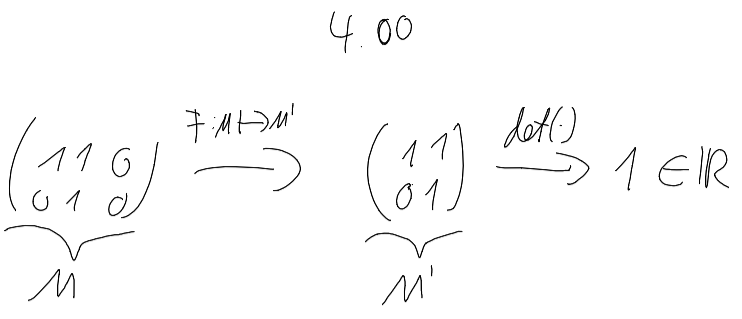
\includegraphics[width=.7\textwidth]{sketch_04_00.png}
        \caption{Sketch 4.00}
    \end{figure}
\end{proof}

\begin{lemma}\label{lem:4.2}\marginnote{The property of full rank is stable under small pertubation!}
    Fix \(F:M^m\to N^n,p\in M\).
    \begin{enumerate}
        \item If \(dF_p\) is injective, then there exists a neighborhood of \(p\) on which 
              \(dF_{\cdot}\) is injective. 
        \item If \(dF_p\) is surjective, then there exists a neighborhood of \(p\) on which 
        \(dF_{\cdot}\) is surjective. 
    \end{enumerate}
\end{lemma}

\begin{proof}
    This is a local statement. We can therefore assume that \(M,N\) are open subsets of \(\R^m,\R^n\) respectively.
    Then \[dF_{(\cdot)}:M\to \Mat(n\times m)\] 
    is smooth, hence continuous. By assumption \(dF_p\in \Mat(n\times m)^{\text{full rank}}\). But \(\Mat(n\times m)^{\text{full rank}}\), so 
    the preimage is open (by lemma \ref{lem:4.1}) and contains \(p\).
\end{proof}

\begin{remark}\marginnote{important: contains both a definition and a counterexample!}
    \begin{enumerate}
        \item If \(F:M\to N\) is both an immersion and a submersion, then we say that \(F\) is a \dhighlight{local diffeomorphism}. We will see (by the rank theorem \ref{thm:4.3})
        that \(F\) is a local diffeomorphism \(\iff\forall p\in M\exists p\in U: F\restrict{U}\) is a diffeomorphism.
        \item be warned. local diffeomorphism need not be global: \begin{alignat*}{10}
            \R^2&\equiv \C\supset& S^1=&\{|z|=1\}\to &S^1\\
            (x,y)&\mapsto x+iy &z&\xmapsto{\phantom{\{|z|=1\}\to}}  &z^2
        \end{alignat*}
    \end{enumerate}
\end{remark}

\begin{definition*}
    An immersion is an \dhighlight{embedding} if it is a homeomorphism onto its image 
    with the subspace topology.
\end{definition*}

\begin{example}
    \begin{figure}[H]
        \centering
        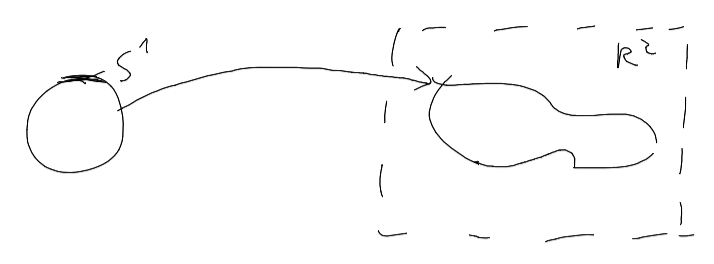
\includegraphics[width=.7\textwidth]{sketch_4_01.png}
        \caption{Sketch 4.01}
    \end{figure}
    Another example: \[S^n=\{(x_0,\dots,x_n)\in\R^{1+n}\mid\sum x_i^2=1\}\subset\R^{1+n}\]
    with \[i:S^n\hookrightarrow \R^{1+n}\]

    \dhighlight{Non-examples}
    \begin{figure}[H]
        \centering
        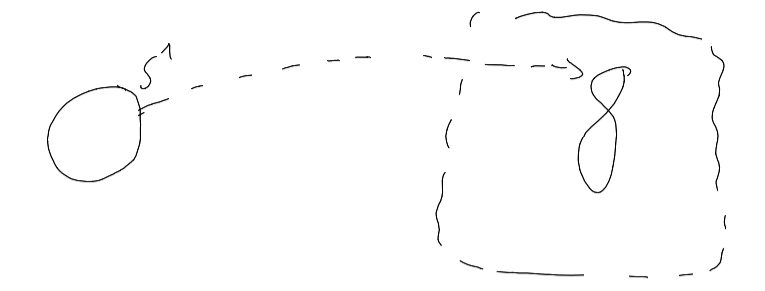
\includegraphics[width=.7\textwidth]{sketch_4_02.png}
        \caption{Sketch 4.02}
    \end{figure}
    parametrized by \[t\mapsto (\sin t,\sin 2t)\]
    and 
    \begin{align*}
        \R&\mapsto \R^2/\Z^2=S^1\times S^1\\
        t&\mapsto (t,\alpha t),\text{   } \alpha \in\R\setminus \Q 
    \end{align*}
    Can show\footnote{not obvious, non-examable} that the image is dense. It is an immersion, but no a homeomorphism!
\end{example}

\markeol{08}
\beginlecture{09}{08.11.2024}

\section{The rank theorem}\marginnote{This is arguably the most important result of the first half of the course. There is a lot of results in \cite{smooth_manifolds}, what is actually useful? Implied answer: Rank theorem}

\begin{theorem}[rank theorem]\label{thm:4.3} Let \(F:M^m\to N^n\) be a smooth map of 
    constant rank \(r\). For each \(p\in M\), there exist charts \((U,\varphi):p\in U\) and \((V,\psi):F(U)\subset V\),
    such that \[\hat{F}\coloneqq \psi \circ F\circ\varphi^{-1}:\]
    \begin{figure}[H]
        \centering
        \caption{Sketch 4.03}
        \(\hat{F}\) takes the form 
        \[\hat{F}(x_1,\dots,x_r,x_{r+1},\dots,x_m)=(x_1,\dots,x_r,0,\dots,0)\]
    \end{figure} 
    
\end{theorem}

\begin{remark}\marginnote{Up to diffeomorphism there is only one map of constant, full, rank}
    By lemma \ref{lem:4.2}, if \(F\) has full rank at \(p\in M\), then 
    \begin{itemize}
        \item  if \(m=r\geq n\), then \(F\) is an submersion near \(p\) and \[\hat{F}(x_1,\dots,x_n,x_{n+1},\dots,x_m)=(x_1,\dots,x_n)\]
        \item \(m=r\leq n\), then \(F\) is an immersion near \(p\), and \[\hat{F}(x_1,\dots,x_m)=(x_1,\dots,x_m,0,\dots,0)\]
        \item \(m=n\implies\) up to the diffeomorphism, \(\hat{F}\) is just the identity
    \end{itemize}
    
\end{remark}

\begin{remark}
    This theorem is a non-linear 
    generalization of the following linear algebra fact: \(L:V^m\to W^n\), then 
    there are linear maps \(\varphi:V^m\stackrel{\simeq}{\to}\R^m,\psi:W^n\stackrel{\simeq}{\to}\R^n\),
    such that \(\hat{L}\coloneqq \psi\circ L\circ \phi^{-1}\) takes the form 
    \[\hat{L}(x_1,\dots,x_r,x_{r+1},\dots,x_m)=(x_1,\dots,x_r,0,\dots,0),\]
    where \(r=\text{rank}(L)\).
\end{remark}

\begin{proof}[Proof of theorem \ref{thm:4.3}]
    \marginnote{see \cite{smooth_manifolds}}
    \dhighlight{Step 0:} We might as well assume that \(M=U\subset \R^m,N=V\subset\R^n\), since we only make a local statement up to diffeomorphism.
    We may also assume, up to reordering the coordinates, that the matrix \((\partial_{x_i}F^j(p))_{1\leq i,j\leq r}\)
    is \dhighlight{invertible} for \(p\in U\). We label our coordinates:\marginnote{source coordinates in \(U\)}  \[(x_1,\dots,x_r,y_1,\dots,y_{m-r})\] 
    \marginpar{Tarkget coordiantes}\[(v_1,\dots,v_r,\dots,w_1,\dots,w_{n-r})\]
    and wlog \(F(0,0)=(0,0)\).

    We write \(F(x,y)=\underbrace{Q(x,y)}_{v\text{-coordinates}},\underbrace{R(x,y)}_{w\text{-coordinates}}\). Notice that \((\partial_{x_i}Q^j)\)
    is non-singular.

    \dhighlight{Step 1:} Define \(\varphi:U\to\R^m,\varphi(x,y)=(Q(x,y),y)\). Then \begin{align*}
        d\varphi_{(0,0)}=\begin{pmatrix}
            \overbrace{\partial_{x_i}Q^j}^{\in \Mat(r\times r)} & \partial_{y_i}Q^j\\
            0 & \underbrace{1}_{\in \Mat((n-r)\times (n-r))}
        \end{pmatrix}
    \end{align*}
    \(\implies\) by the inverse function theorem, there  exist connected neighborhoods \(U_0\subset U,\tilde{U_0}\subset \in \Mat((n-r)\times (n-r))\varphi(U)\),
    such that \(\varphi\restrict{U_0}:U_0\to\tilde{U_0}\). We may as well assume that \(\tilde{U_0}\) is a cube, i.e. \((-\epsilon,\epsilon)^n\).
    \begin{figure}[H]
        \centering
        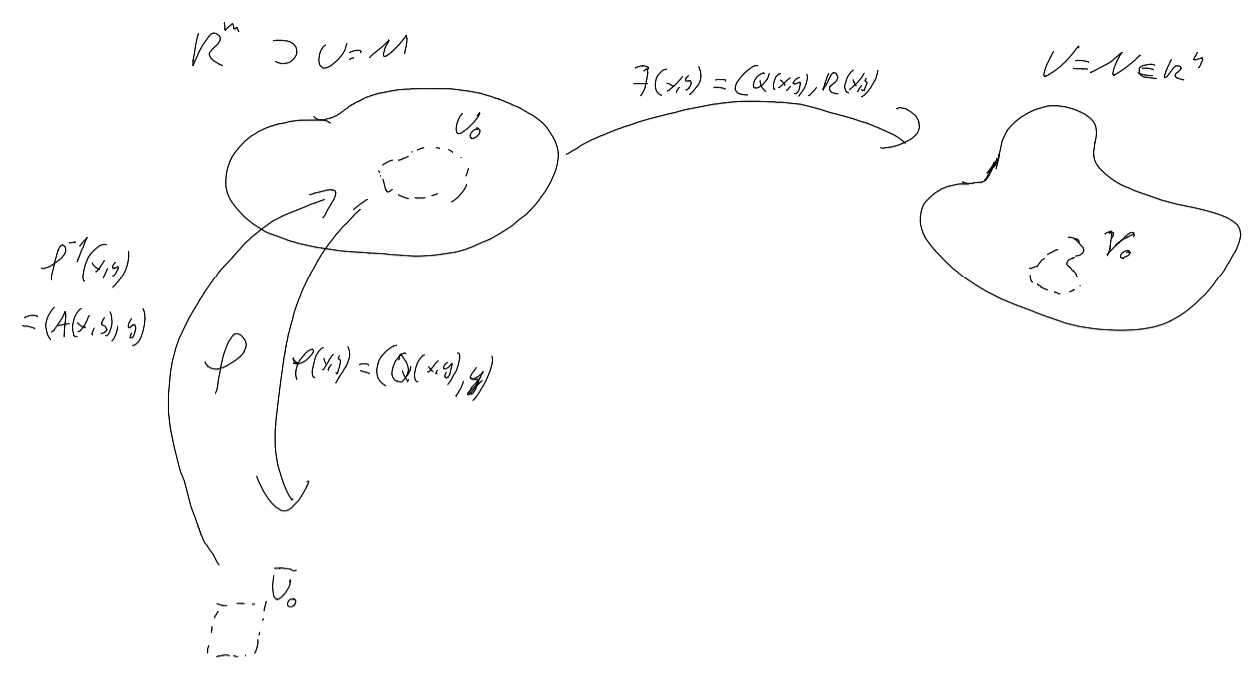
\includegraphics[width=.7\textwidth]{sketch_4_04.png}
        \caption{Sketch 4.04}
    \end{figure}
    While \(\varphi^{-1}(x,y)=(A(x,y),B(x,y))\), for some \(A:\tilde{U_0}\to\R^r\), \(B:\tilde{U_0}\to\R^{m-r}\).
    We compute \begin{align*}
        (x,y)=\varphi\circ\varphi^{-1}(x,y)=\varphi\left(A(x,y),B(x,y)\right)=(Q(A(x,y),B(x,y)),B(x,y))\implies \substack{x=Q(A(x,y),B(x,y))\\y=B(x,y)}
    \end{align*}
    Hence \highlight{\(\varphi^{-1}(x,y)=(A(x,y),y)\)}.

    \dhighlight{Step 2:} Observe that 
    \[F\circ \varphi^{-1}(x,y)=(Q(\varphi^{-1}(x,y)),R(\varphi^{-1}(x,y)))=(x,\tilde{R}(x,y)),\]
    where \[\tilde{R}(x,y)=R(\varphi^{-1}(x,y)).\]
    Then \begin{align*}
        d(F\circ\varphi^{-1})=\begin{pmatrix}
            \overbrace{1}^{\in \Mat(r\times r)} & 0 \\
            \partial_{x_i}\tilde{R}(x,y)^j& \underbrace{\partial_{y_i} \tilde{R}^j}_{\in\Mat((m-r)\times (m-r))}
        \end{pmatrix}
    \end{align*}
    But the rank of \(d(F\circ \varphi^{-1})\) is \(r\), because \(\varphi^{-1}\) is a diffeomorphism and \(F\) has rank \(r\)
    \begin{itemize}
        \item Since \(1_{r\times r}\) has rank \(r\), we must have \(\partial_{y_i}\tilde{R}\equiv 0\)
    \end{itemize}
    We write \(S(x)\coloneqq \tilde{R}(x,y)\), we now have \begin{equation}\label{eq:proof_rank_thm}F\circ\varphi^{-1}(x,y)=(x,S(x))\end{equation}.\marginnote{to make clear \(\tilde{R}\) does not really depend on \(y\)}

    \dhighlight{Step 3:} Recall
    \begin{align*}
        F:U&\to V\subset\R^n\\
        F(0,0)&=(0,0)
    \end{align*} 
    Let \(V_0\subset V\) be defined as follows:
    \begin{align*}
        V_0\coloneqq \{(v,w)\in V\mid (v,0)\in \tilde{U}_0\}
    \end{align*}
    By (\ref{eq:proof_rank_thm}), \(F\circ \varphi^{-1}(\tilde{U}_0)\subset V_0\). Hence \(F(U_0)\subset V_0\).
    Set \(\psi:V_0\to\R^n,\psi(v,w)=(v,w-S(v))\)\marginnote{\(S(v)\) makes perfect sense, since both \(x,v\) have \(r\) entries}.
    Clearly \(\psi\) is a diffeomorphism, since\[(v,w)\mapsto (v,w+S(w))\]
    is am inverse. \(\implies (V_0,\psi)\) is a smooth chart. 
    \[\hat{F}\coloneqq \psi\circ F\circ \phi^{-1}=\Psi(x,S(x))=(x,S(x)-S(x))=(x,0)\qedhere\]
\end{proof}

\begin{remark}
    This is one theorem you should really not forget! If you continue to think about Manifolds in your life, this is really useful! %TODO: Quote
    Do not remember the proof, remember the statement!
\end{remark}










